\section{Синтетический контроль}
\begin{frame}{Что если общего тренда нет: ограничения продажи табака в Калифорнии\footcite{abadie2010synthetic}}
\begin{figure}
    \centering
    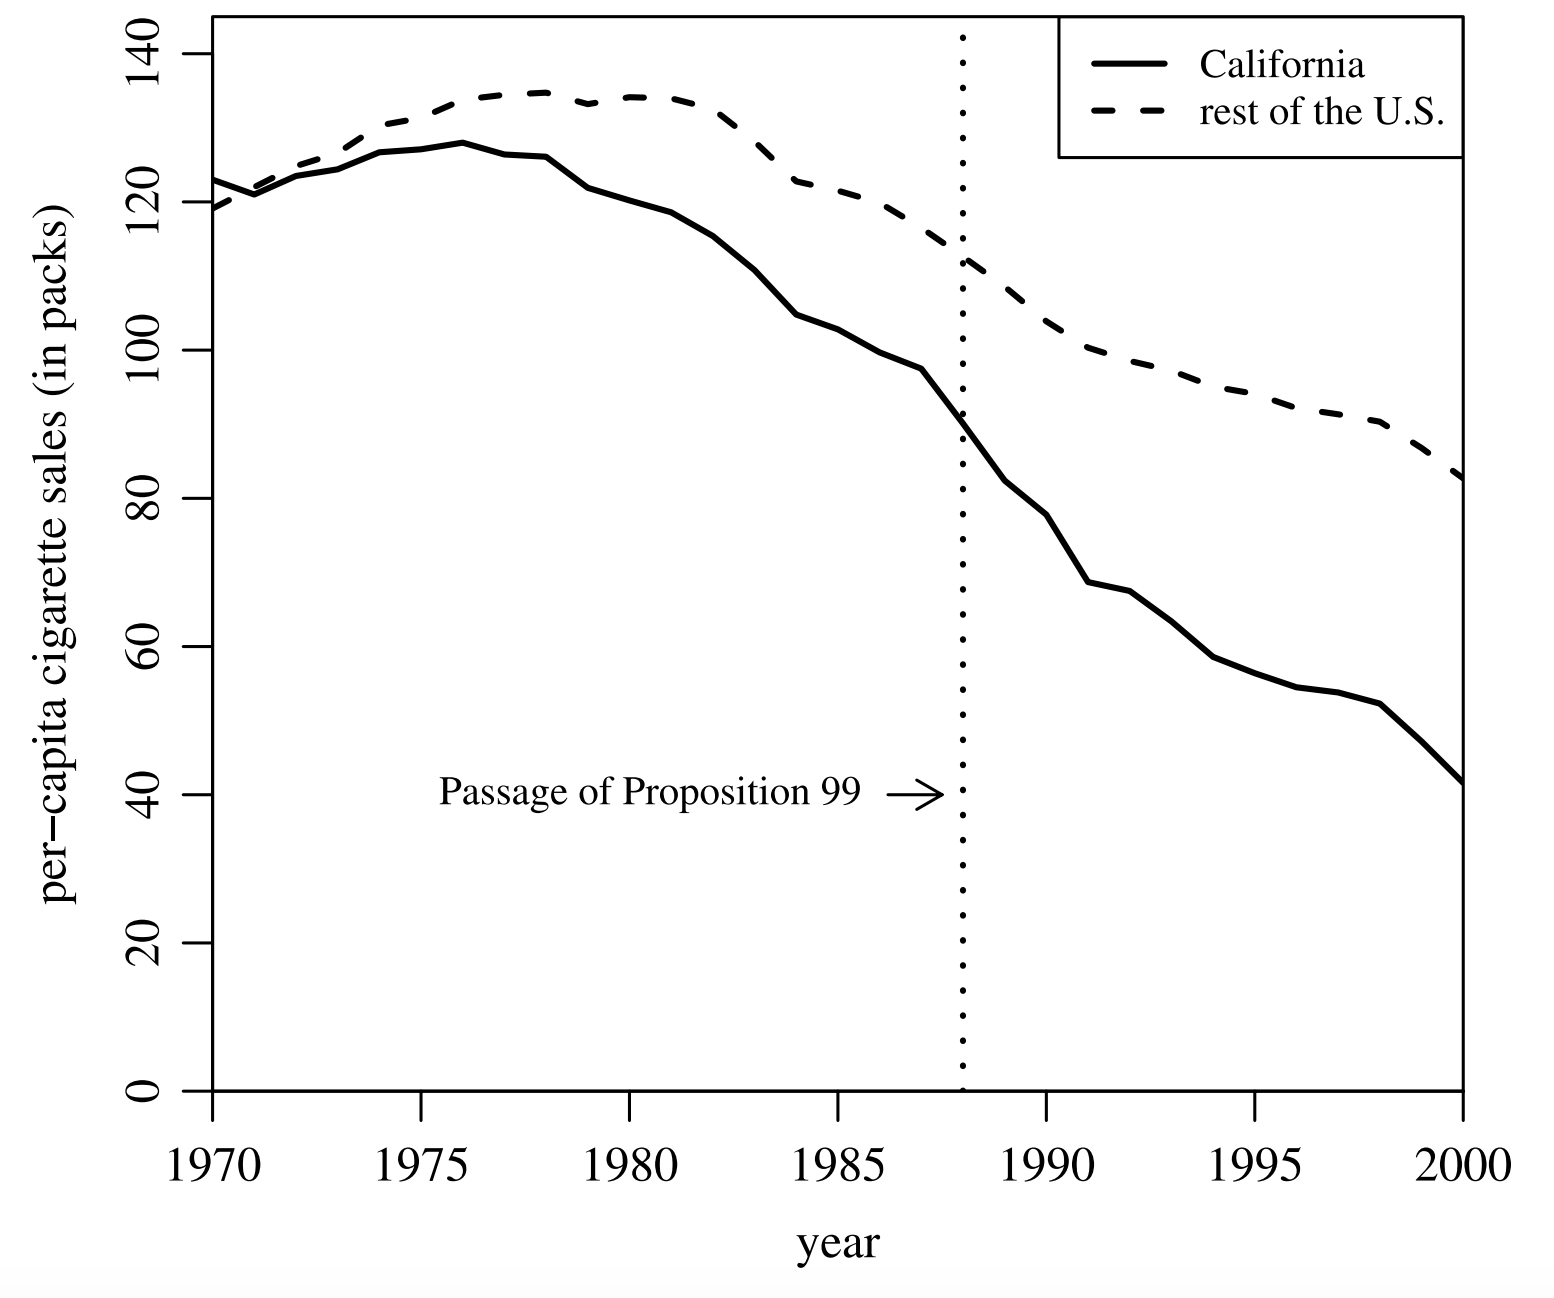
\includegraphics[width=0.8\textwidth]{Images/california_basic.png}
\end{figure}
\end{frame}

\begin{frame}{Обсуждение предпосылок}
    \begin{itemize}[<+->]
        \item Пока будем рассматривать кейс с одним объектом воздействия
        \item Почему тренды различаются?
        \item Наблюдаемые факторы $X_i$ меняются
        \item Ненаблюдаемые факторы $\mu_i$ тоже меняются
    \end{itemize}
    
    \pause
    Итоговая модель:
    $$Y^0_{it} = \delta_i + X_i^T\beta_t + \lambda^T_t\mu_i + \varepsilon_{it}$$
    
    \pause
    Чем она отличается от модели из diff-in-diff?
\end{frame}


\begin{frame}{Синтетический контроль}
    \begin{itemize}[<+->]
        \item Мы можем оценить эту модель напрямую и сделать difference-in-difference с контролем
        \item Эффективнее найти веса:
        $$\hat Y_{0t} = \sum^N_iw_iY_{it} = \delta_0\sum^N_iw_i + \left(\sum^N_iw_iX_i\right)^T\beta_t + \\ \lambda^T_t\left(\sum^N_iw_\mu_i\right) + \sum^N_iw_i\varepsilon_{it}$$
    \end{itemize}
\end{frame}


\begin{frame}{Поиск весов}
    \begin{itemize}
        \item $\sum^N_iw_i = 1$
        \item $\sum^N_iw_iX_i = X_0$
        \item $\sum^N_iw_i\mu_i = \mu_0$
        \pause
        \item<+-> или
    \end{itemize}
    \pause
    \begin{itemize}
        \item $\sum^N_iw_i = 1$
        \item $\sum^N_iw_iX_i = X_0$
        \item $\sum^N_iw_iY_i = Y_0$
    \end{itemize}
    
    \pause
    % Как искать веса?
    % \begin{itemize}[<+->]
    %     \item Что если вариантов несколько?
    %     \item Что если система не имеет решения?
    %     \item Как построить доверительный интервал?
    % \end{itemize}
\end{frame}


\begin{frame}{Синтетический контроль}
\begin{figure}
    \centering
    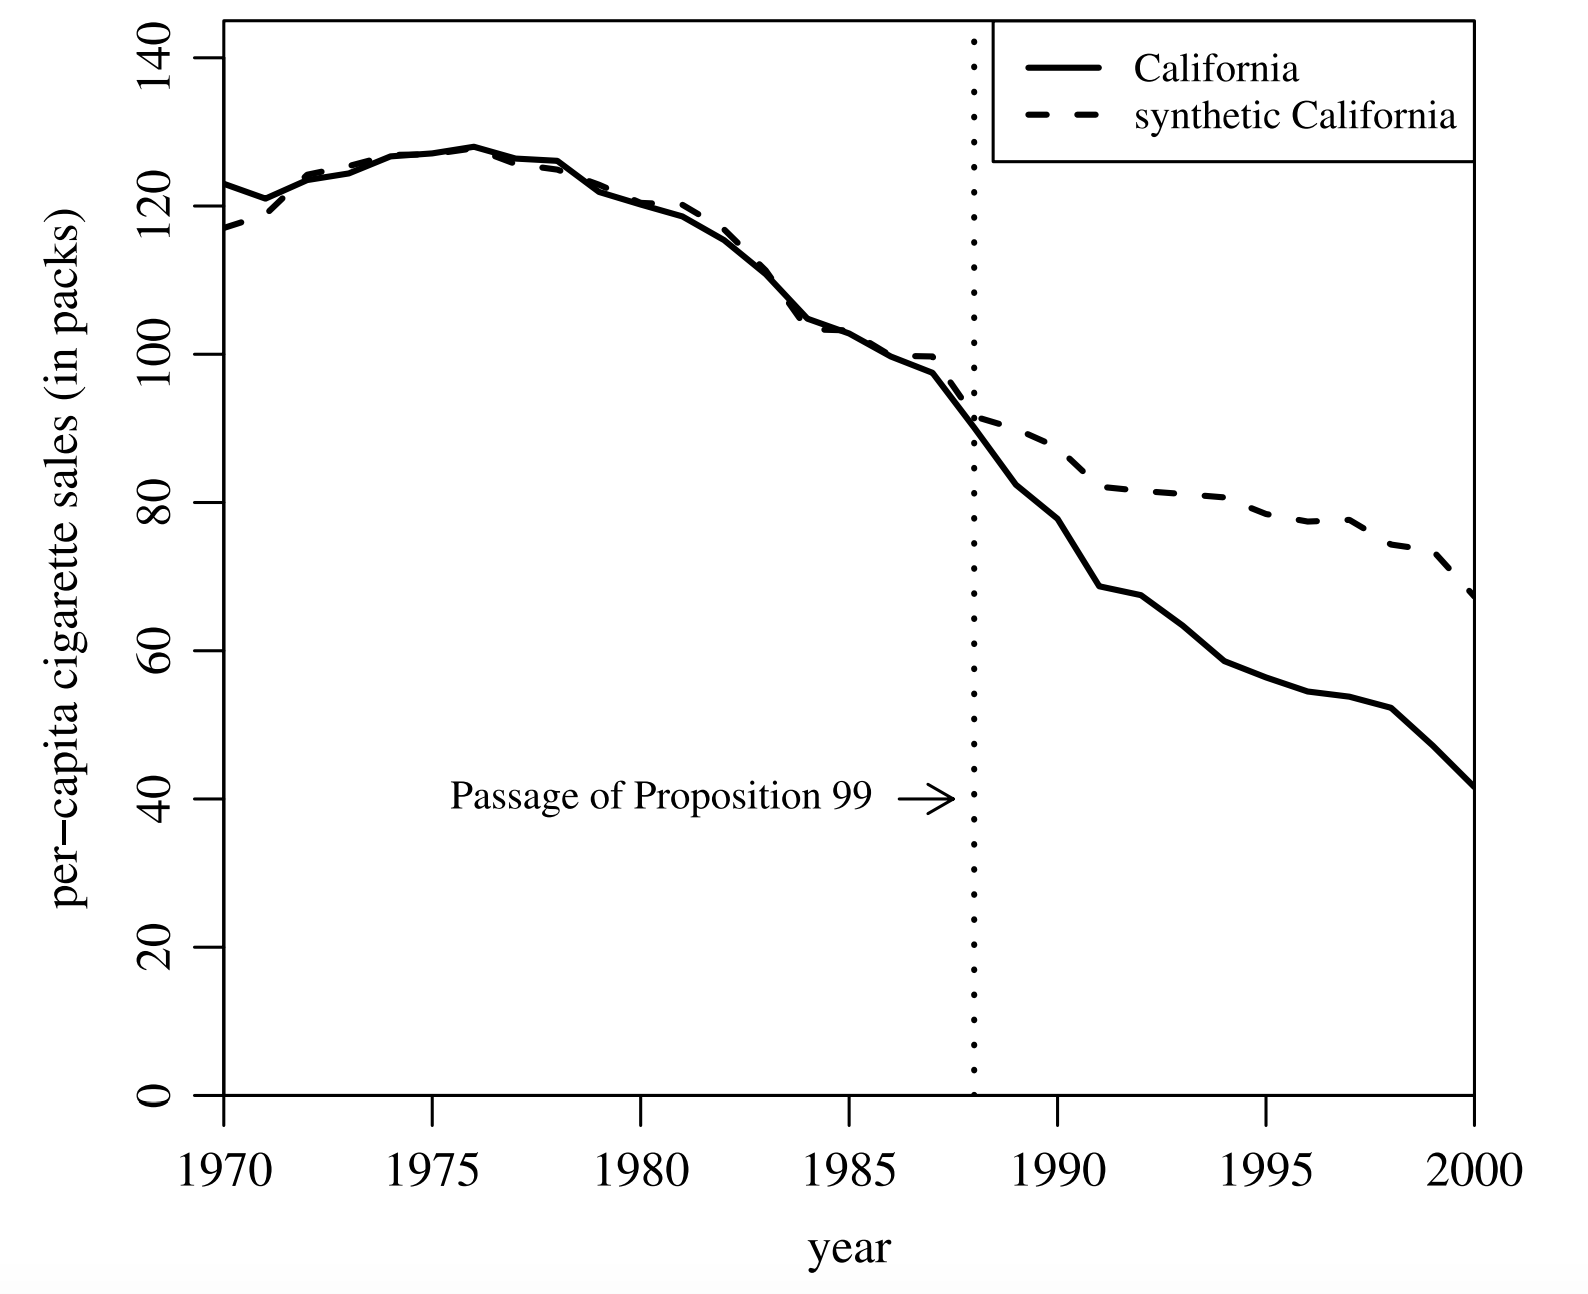
\includegraphics[width=0.8\textwidth]{Images/california_synth.png}
\end{figure}
\end{frame}

\begin{frame}{Для других штатов}
\begin{figure}
    \centering
    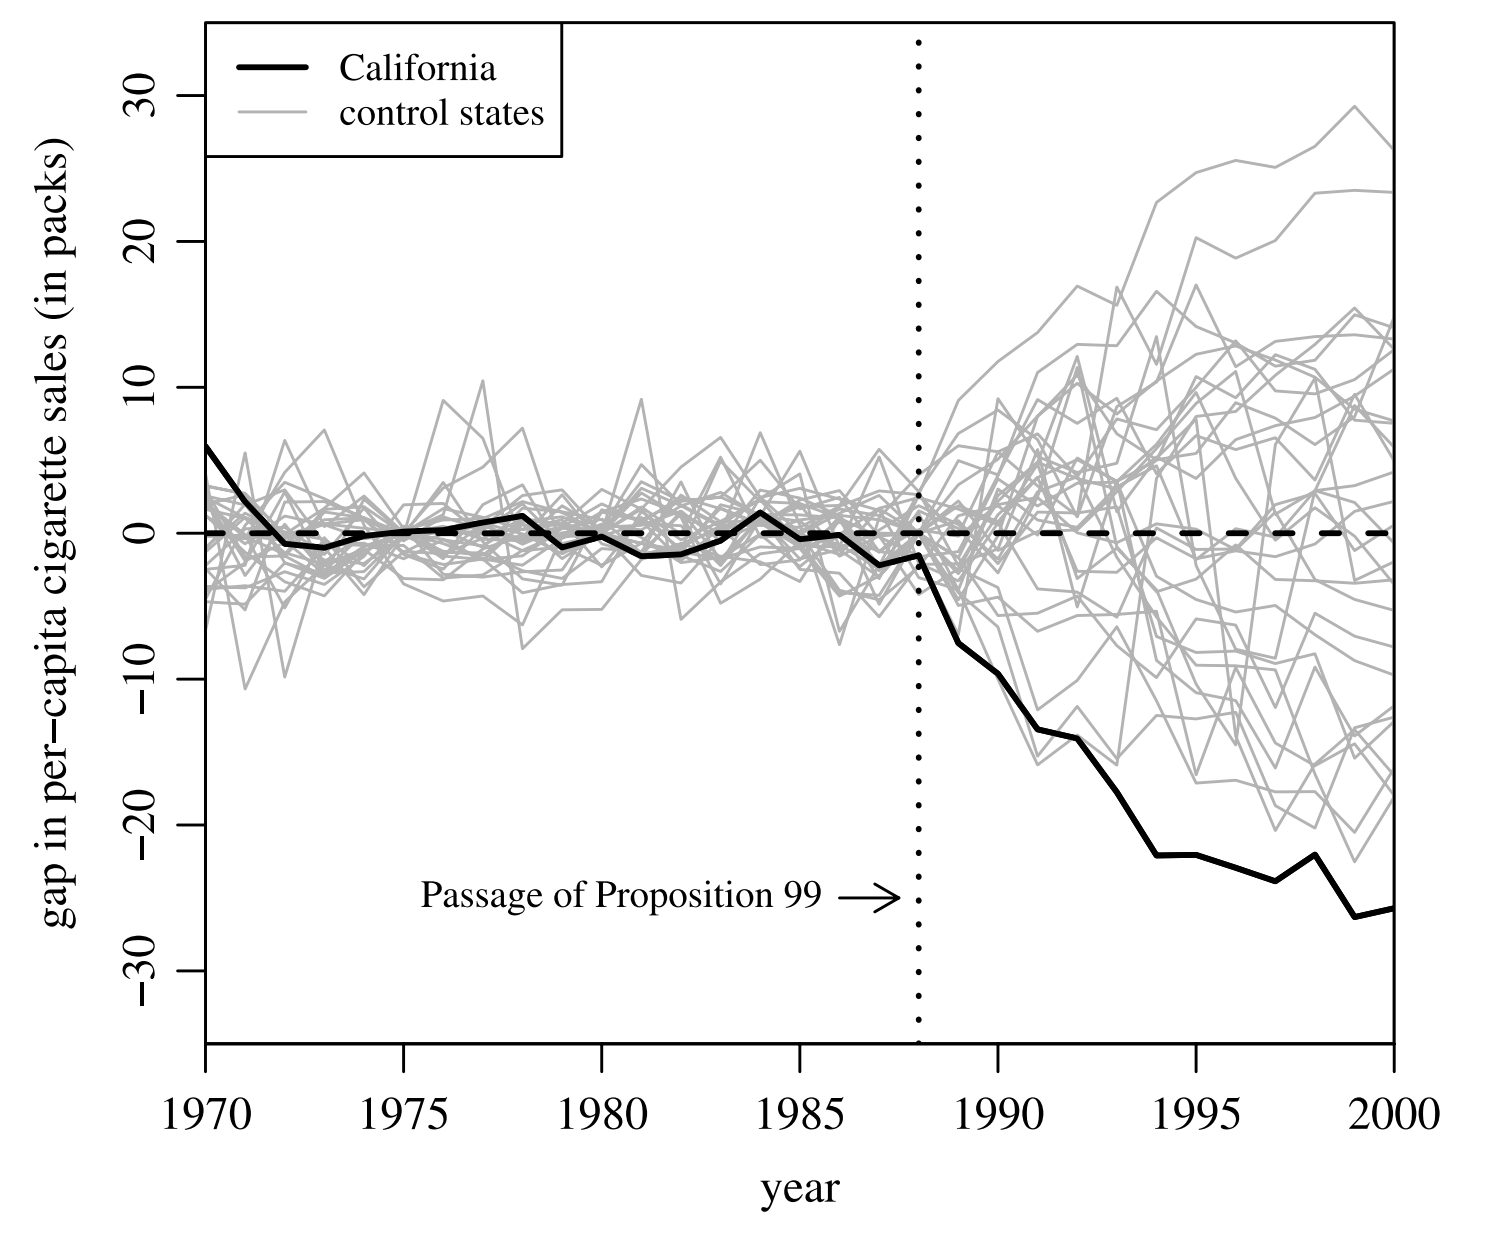
\includegraphics[width=0.8\textwidth]{Images/california_placebo.png}
\end{figure}
\end{frame}

\section{Примеры}
\begin{frame}{Еще пример: объединение Германии\footcite{abadie2015comparative}}
    \begin{figure}
        \centering
        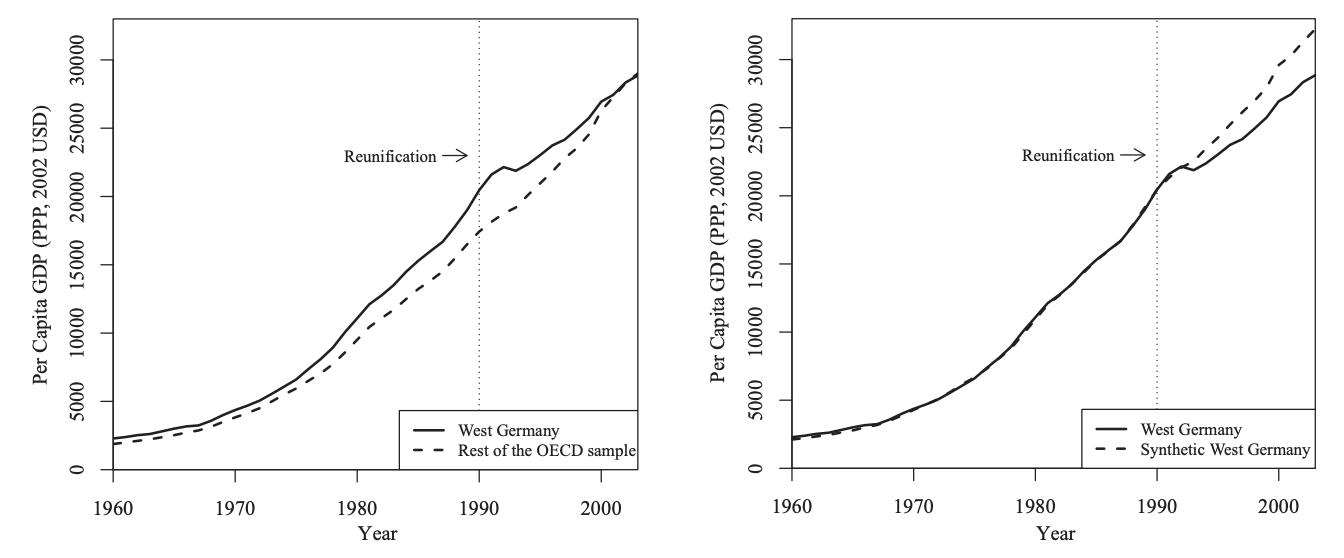
\includegraphics[width=\textwidth]{Images/germany_basic.png}
    \end{figure}
\end{frame}

\begin{frame}{Плацебо тест 1}
    \begin{figure}
        \centering
        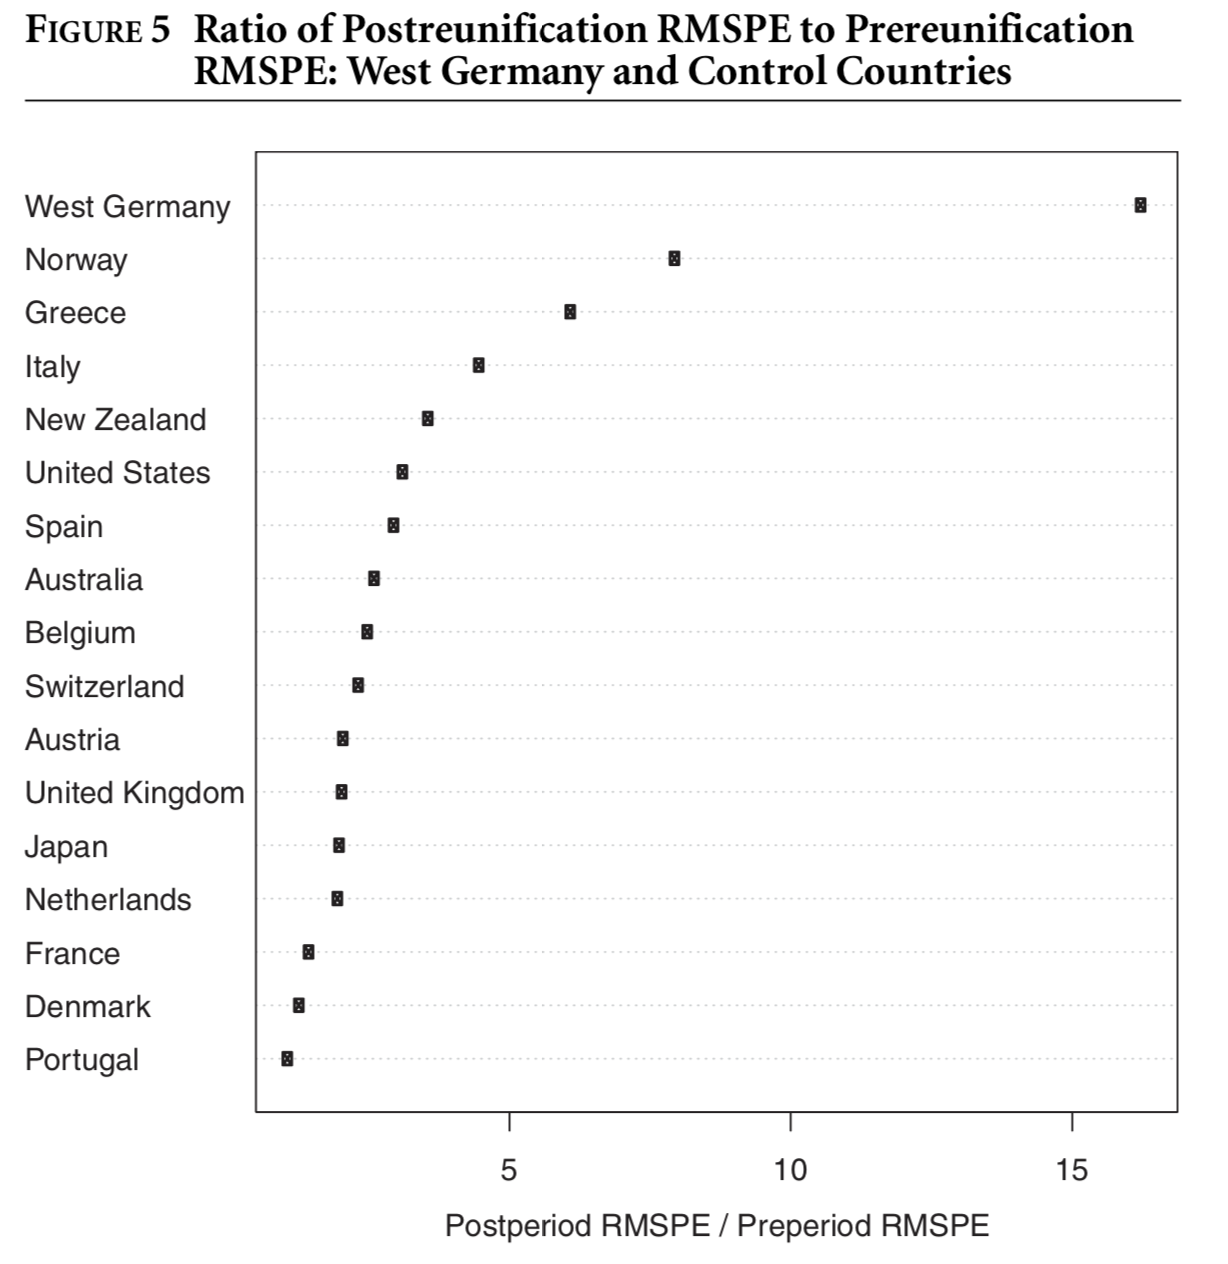
\includegraphics[width=0.8\textwidth]{Images/germany_placebo.png}
    \end{figure}
\end{frame}


\begin{frame}{Плацебо тест 2}
    \begin{figure}
        \centering
        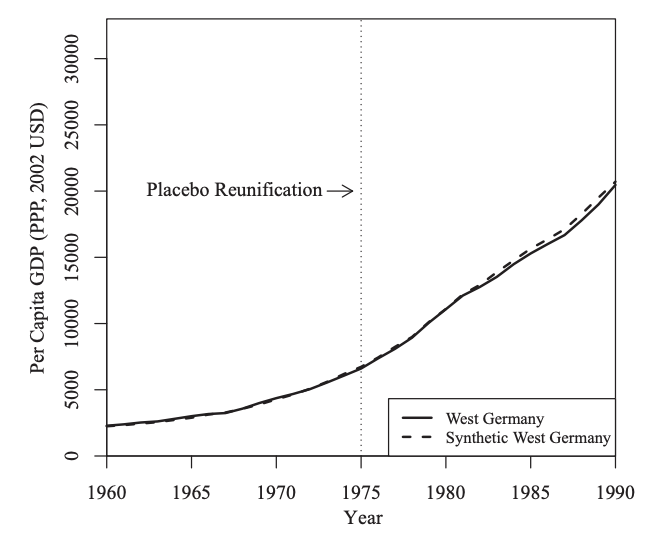
\includegraphics[width=\textwidth]{Images/germany_placebo2.png}
    \end{figure}
\end{frame}


% \begin{frame}{Обобщение}
%     \item Можно обобщить на несколько объектов воздействия
% \end{frame}


% Xu Y. Generalized synthetic control method: Causal inference with interactive fixed effects models //Political Analysis. – 2017. – Т. 25. – №. 1. – С. 57-76.